
\section{git用法}

\begin{figure}[htpb]
    \begin{center}
        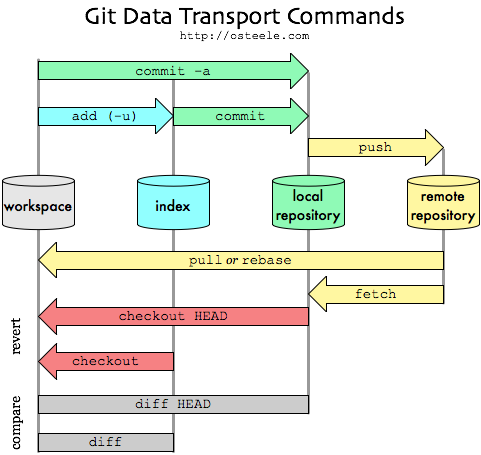
\includegraphics[keepaspectratio,width=0.5\paperwidth]{Pictures/git_dataflow.png}
    \end{center}
    \caption{Git数据流}
\end{figure}

\subsection{配置}
配置彩色界面,commit操作的默认编辑器
\begin{verbatim}
git config --global color.ui true
git config --global core.editor "vim"
\end{verbatim}

\subsection{基本用法}
创建版本库

\begin{verbatim}
git init
\end{verbatim}

添加文件并提交

\begin{verbatim}
git add -A
git commit -m ``initialized''
\end{verbatim}


修改文件并提交
\begin{verbatim}
git commit -a
\end{verbatim}

撤销工作区修改
\begin{verbatim}
git checkout -- . 撤销修改,用暂存区覆盖工作区
git checkout .  同上
\end{verbatim}

查看历史
\begin{verbatim}
git log <refs>本分支提交历史
git log -3 只显示最近3次提交
git log --stat 显示修改统计
git reflog [show] <refs> 引用历史
\end{verbatim}

查看文件状态
\begin{verbatim}
git checkout [HEAD] 显示工作区、暂存区、HEAD之间的差异
git status
git ls-files [-c] 查看暂存区文件
git ls-files -m 查看被修改的文件
git ls-files -d 查看被删除的文件
git ls-files -o 查看其他文件,即未被追踪的文件
git write tree; git ls-tree <treeish> 查看tree包含的blob
\end{verbatim}

检出历史文件
\begin{verbatim}
git checkout <commit> [--] filename
省略commit,则表示暂存区。
\end{verbatim}

整体回归历史
\begin{verbatim}
git reset --hard <id> 
提交日志也会一起回归历史
git checkout <id> 
会进入分离头指针状态,此后的提交日志不容易查看
git checkout -b <new_branch> <id>
新建分支,回归历史
\end{verbatim}
总之,checkout命令修改HEAD指向,reset修改分支指向

修改刚才的提交的提交说明
\begin{verbatim}
git commit --amend
\end{verbatim}

修改某个历史提交的提交说明
\begin{verbatim}
git rebase -i <some history>
\end{verbatim}

将从v1开始的历次提交逐一导出为补丁
\begin{verbatim}
git format-patch v1..HEAD
\end{verbatim}

不慎提交了不想提交的文件,如winxp.img
\begin{verbatim}
git rm --cached winxp.img
git commit --amend
\end{verbatim}
git rm将文件从工作区和index同时删除。--cache指定不从工作区删除。

比较差异:
比较工作区和暂存区:git diff
比较工作区与HEAD:git diff HEAD
比较工作区与里程碑A:git diff A
比较暂存区与里程碑A:git diff --cached A
比较暂存区与HEAD:git diff --cached
比较里程碑A和B git diff B A

\subsection{显示id}
\begin{verbatim}
git rev-parse master
\end{verbatim}

创建里程碑``v1''
\begin{verbatim}
git tag v1
\end{verbatim}

\subsection{GitHub操作}
\begin{verbatim}
git clone https://github.com/allset1987/YHTravelAssistant.git
//do some modification and commit
git pull
git push
\end{verbatim}

\subsection{Google Hosting操作}
在网页端建立项目,本地端在~/.netrc文件中添加用户名和密码配置:
\begin{verbatim}
machine code.google.com login lmz0610@gmail.com password [generated googlecode.com password] 
\end{verbatim}

clone项目时不要带用户名和密码。Google Codes目前只支持HTTPS方式使用git。
\begin{verbatim}
git clone https://code.google.com/p/technotes-gh/
\end{verbatim}

如果需要将已有的版本库提交到服务器,则配置remote信息,给remote取名(如origin),如:
\begin{verbatim}
git remote add origin https://code.google.com/p/sysnetwork-tools/
\end{verbatim}

首次提交时,如果服务器端为空,还没有master分支,则push时应指定分支和remote名
\begin{verbatim}
git push origin master 
\end{verbatim}
此后push操作只需要
\begin{verbatim}
git push
\end{verbatim}

